\documentclass[../Main.tex]{subfiles}
\usepackage{tabularx}
\begin{document}
\section{Khảo sát}
Để có cái nhìn khách quan cũng như có trải nghiệm thực tế để xây dựng một ứng dụng quản lí đồ án Android em đã khảo sát qua một số ứng dụng: Trello, Asana, Any.Do, eHUST.

Sau khi trải nghiệm các ứng dụng thì em nhận thấy nhìn chung tất cả các ứng dụng đều có giao diện rất thân thiện với người dùng. Về Trello thông qua khảo sát em thấy ứng dụng này hướng đến sự đơn giản, linh hoạt, miễn phí, nó thu hút được khoảng 4.6 triệu người đăng kí sử dụng, tuy nhiên em nhận thấy nó có một nhược điểm cho là đối với các thiết bị như smart phone thì màn hình của điện thoại không được rộng nên việc sử dụng tay để kéo thả các task là không hợp lí, nó chỉ hợp lí và đẹp trên các thiết bị có màn hình rộng hơn như ipad hay dùng với bản web, các tính năng của Trello rất hữu ích nó là một công cụ quản lí công việc trực quan hỗ trợ các nhóm lên ý tưởng, lập kế hoạch một cách hiệu quả, có tổ chức.

Khác với Trello thì Asana không trực quan hoá luồng công việc mà nó trông giống với một danh sách các công việc cần phải làm, nơi tất cả mọi người có thể tạo nhiệm vụ và giao việc cho người khác, giúp người quản lí có thể theo dõi tổng quan được dự án, các công việc được sắp xếp theo độ ưu tiên giúp cho người thực hiện dế dàng có thể nhận biết các công việc nào cần thực hiện trước, sau. 

Về Any.Do là phần mềm mang lại trải nghiệm khá tuyệt vời cho em. Nó có giao diện tinh tế, hiện đại, có thể sắp xếp công việc theo độ ưu tiên, có thể thực hiện ghi chú bằng âm thanh hoặc hình ảnh rất sống động, tuy nhiên Any.Do lại không hỗ trợ với ứng dụng thứ 3 như Gmail.

eHUST là một phần mềm dành cho cả sinh viên, giảng viên, cán bộ toàn trường. Với ứng dụng này người dùng có khả năng truy cập và khai thác các thông tin một cách hiệu quá: các thông tin về lớp học, thời khoá biểu, tra cứu sinh viên, giảng viên, nhắc lịch học. Tuy nhiên phần mềm này còn khá là hạn chế và đôi lúc xảy ra sai sót trong quá trình nhắc lịch học cho các bạn sinh viên. 

Thông qua việc khảo sát 4 ứng dụng trên em đã quyết định phát triển ứng dụng "Quản lí đồ án trên nền tảng Android" giúp cho sinh viên, giảng viên có thể quản lí công việc một cách khoa học, giảng viên có thể sát sao hơn với quá trình làm đồ án của sinh viên. Ứng dụng cho phép người dùng có thể tạo công việc, cập nhật công việc, gửi thông báo đến giảng viên khi có bất cứ một sự cập nhật công việc nào đến từ sinh viên, giảng viên cũng có thể tạo lịch gặp mặt để trao đổi trực tiếp với sinh viên, quản trị viên có thể phân công hướng dẫn đồ án. Bên cạnh các chức năng chính trên, ứng dụng cũng cho phép sinh viên, giảng viên xem các tin tức, thông báo quan trọng từ trường, xem thời khoá biểu, tra cứu sinh viên, giảng viên, lớp học. 
\section{Tổng quan chức năng}
\subsection{Biểu đồ use case tổng quát}
Hệ thống bao gồm 3 tác nhân:

\textbf{Sinh viên:} Là đối tượng đã có tài khoản và đăng nhập thành công vào hệ thống.

\textbf{Giảng viên:} Là đối tượng đã có tài khoản đăng nhập thành công trên hệ thống, có các chức năng xem danh sách sinh viên hướng dẫn, quản lí đồ án, xem danh sách lớp trong kì...

\textbf{Quản trị viên:} Là đối tượng đã đăng nhập thành công vào hệ thống với vai trò quản trị có chức năng phân công sinh viên cho giảng viên bất kì.

\begin{figure}[H]
    \centering
    \includegraphics[width=1\linewidth]{Figure/use_case_tổng_quan.png}
    \caption{Sơ đồ use case tổng quan}
    \label{fig:use_case_tổng_quan}
\end{figure}
\newpage
\subsection{Phân rã use case Xem chi tiết công việc}
\begin{figure}[H]
    \centering
    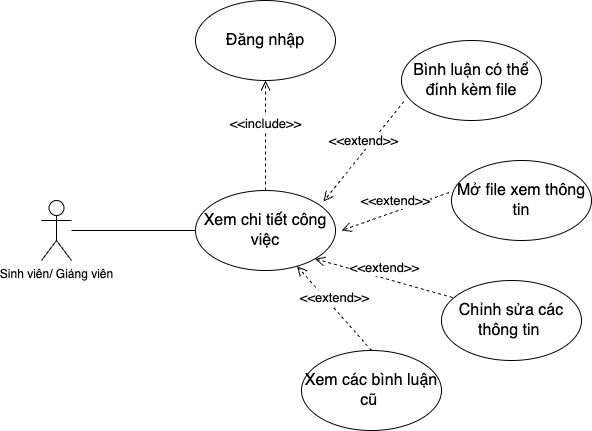
\includegraphics[width=0.85\linewidth]{Figure/use_case_chi_tiet_cv (1).png}
    \caption{Phân rã use case Xem chi tiết công việc}
   \label{fig:use_case_tim_kiem}
\end{figure}

\subsection{Phân rã use case Tìm kiếm người dùng}

\begin{figure}[H]
    \centering
    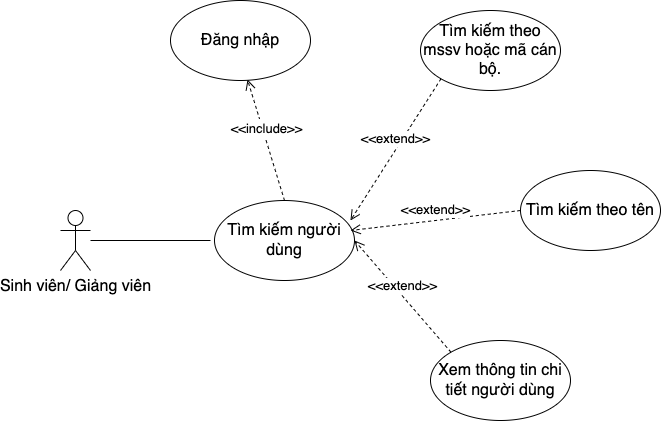
\includegraphics[width=0.9\linewidth]{Figure/use_case_tim_kiem.png}
    \caption{Phân rã use case Tìm kiếm người dùng}
   \label{fig:use_case_tim_kiem}
\end{figure}

\newpage
\subsection{Phân rã use case Bình luận vào công việc}
\begin{figure}[H]
    \centering
    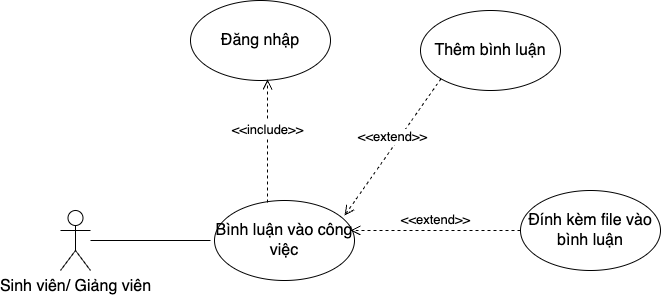
\includegraphics[width=0.8\linewidth]{Figure/use_case_binh_luan_task.png}
    \caption{Phân rã use case Bình luận vào công việc}
    \label{fig:use_case_binh_luan_task}
\end{figure}

\subsection{Phân rã use case Xem danh sách phân công đồ án}
\begin{figure}[H]
    \centering
    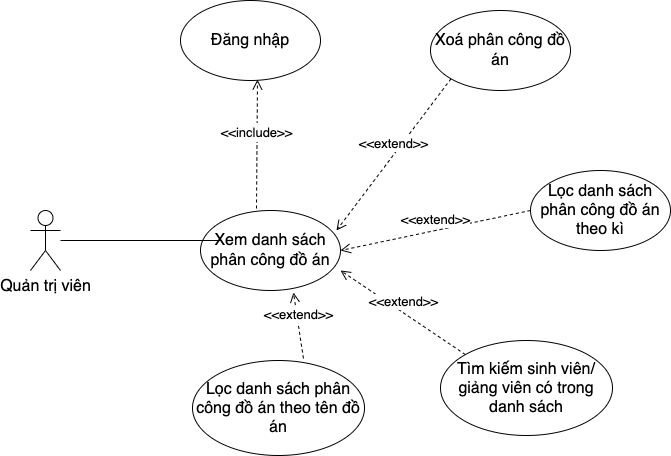
\includegraphics[width=0.75\linewidth]{Figure/use_case_xem_ds_phan_cong.png}
    \caption{Phân rã use case Xem danh sách phân công đồ án}
    \label{fig:use_case_xem_ds_phan_cong}
\end{figure}

\subsection{Phân rã use case Xem file đính kèm}

\begin{figure}[H]
   \centering
    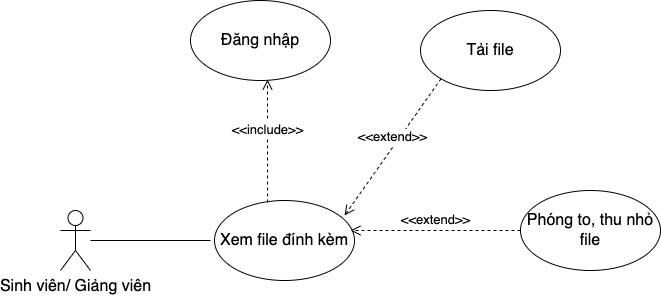
\includegraphics[width=0.75\linewidth]{Figure/use_case_xem_file_dinh_kem.png}
    \caption{Phân rã use case Xem file đính kèm}
    \label{fig:use_case_xem_file_dinh_kem}
\end{figure}


\subsection{Phân rã use case Xem danh sách đồ án hướng dẫn theo kì}
\begin{figure}[H]
    \centering
    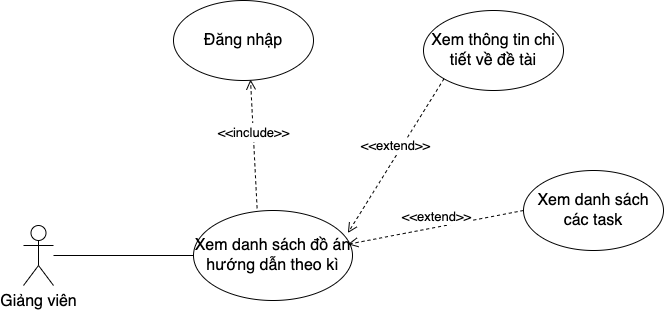
\includegraphics[width=0.8\linewidth]{Figure/use_case_xem_ds_do_an.png}
    \caption{Phân rã use case Xem danh sách đồ án hướng dẫn theo kì}
    \label{fig:use_case_xem_ds_do_an}
\end{figure}                                                                              

\section{Các quy trình nghiệp vụ}

\subsection{Nghiệp vụ Đăng nhập}
\begin{figure}[H]
   \centering
    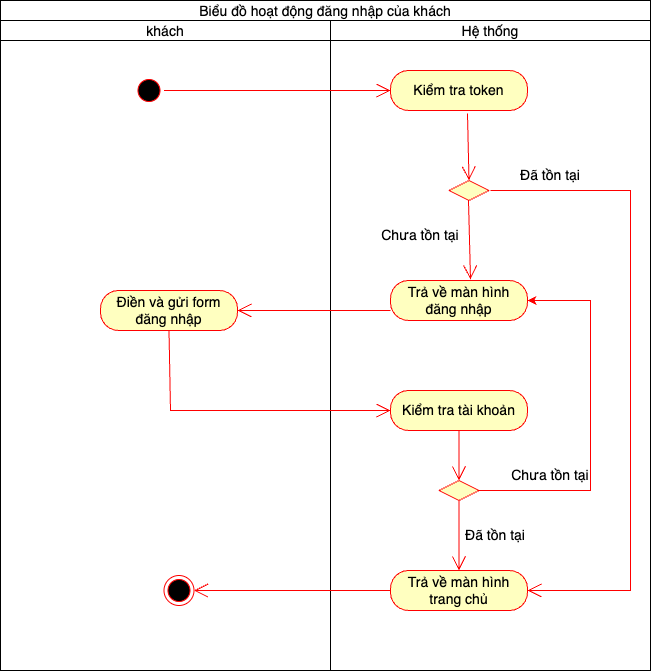
\includegraphics[width=0.85\linewidth]{Figure/dang_nhap.png}
    \caption{Sơ đồ hoạt động quy trình nghiệp vụ Đăng nhập}
    \label{fig:dang_nhap}
\end{figure}
\newpage
\subsection{Nghiệp vụ Tạo công việc}

\begin{figure}[H]
   \centering
    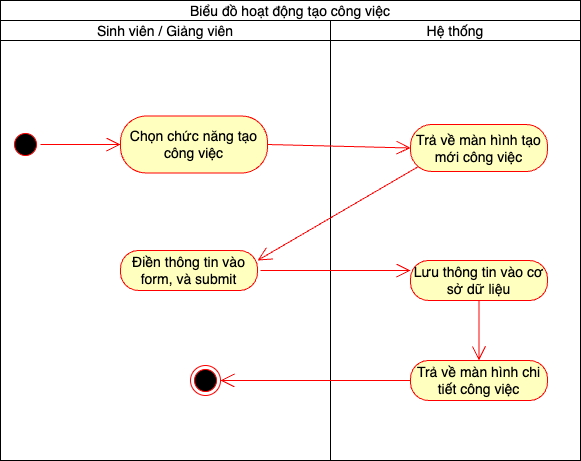
\includegraphics[width=0.85\linewidth]{Figure/qt_new_task.png}
    \caption{Sơ đồ hoạt động quy trình nghiệp vụ Tạo công việc}
    \label{fig:qt_new_task}
\end{figure}

\subsection{Nghiệp vụ Chỉnh sửa công việc}

\begin{figure}[H]
   \centering
    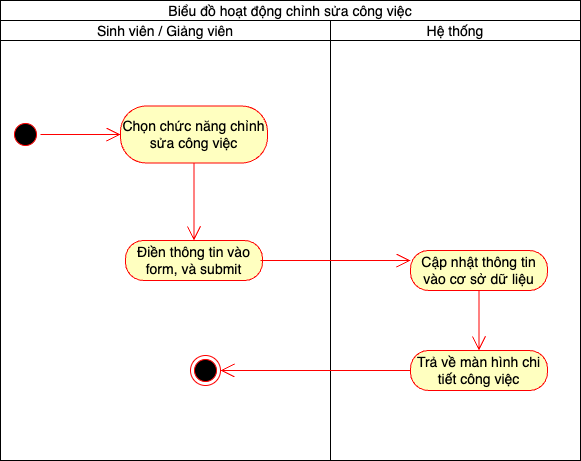
\includegraphics[width=0.85\linewidth]{Figure/qt_edi_task.png}
    \caption{Sơ đồ hoạt động quy trình nghiệp vụ Chỉnh sửa công việc}
    \label{fig:qt_edi_task}
\end{figure} \newpage
\subsection{Nghiệp vụ Bình luận công việc}
\begin{figure}[H]
   \centering
    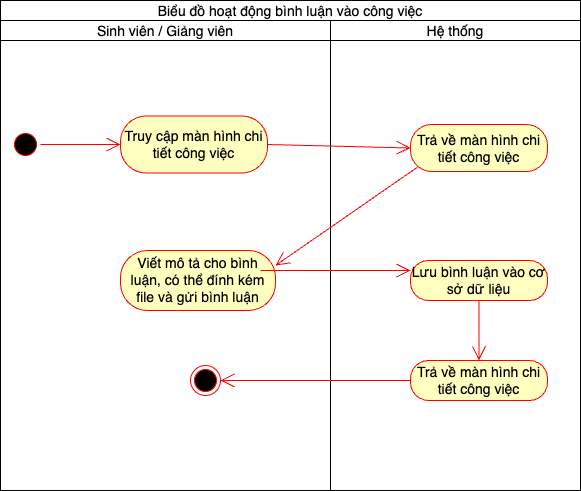
\includegraphics[width=0.85\linewidth]{Figure/qt_cmt.png}
    \caption{Sơ đồ hoạt động quy trình nghiệp vụ Bình luận công việc}
    \label{fig:qt_cmt}
\end{figure}
\subsection{Nghiệp vụ Xoá thông báo đồ án đã đọc}
\begin{figure}[H]
   \centering
    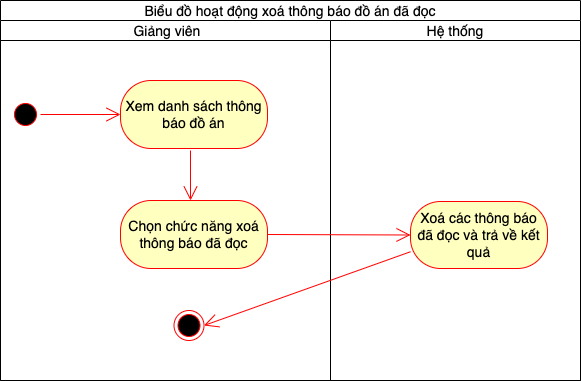
\includegraphics[width=0.85\linewidth]{Figure/qt_xoa_thong_bao.png}
    \caption{Sơ đồ hoạt động quy trình Xoá thông báo đồ án đã đọc}
    \label{fig:qt_xoa_thong_bao}
\end{figure}
\newpage
\subsection{Nghiệp vụ Tạo lịch gặp sinh viên}
\begin{figure}[H]
   \centering
    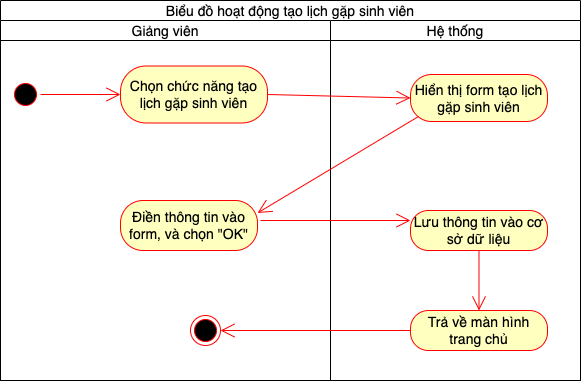
\includegraphics[width=0.75\linewidth]{Figure/qt_meeting.png}
    \caption{Sơ đồ hoạt động quy trình nghiệp vụ Tạo lịch gặp sinh viên}
    \label{fig:qt_meeting}
\end{figure}

\subsection{Nghiệp vụ Phân công hướng dẫn đồ án}
\begin{figure}[H]
   \centering
    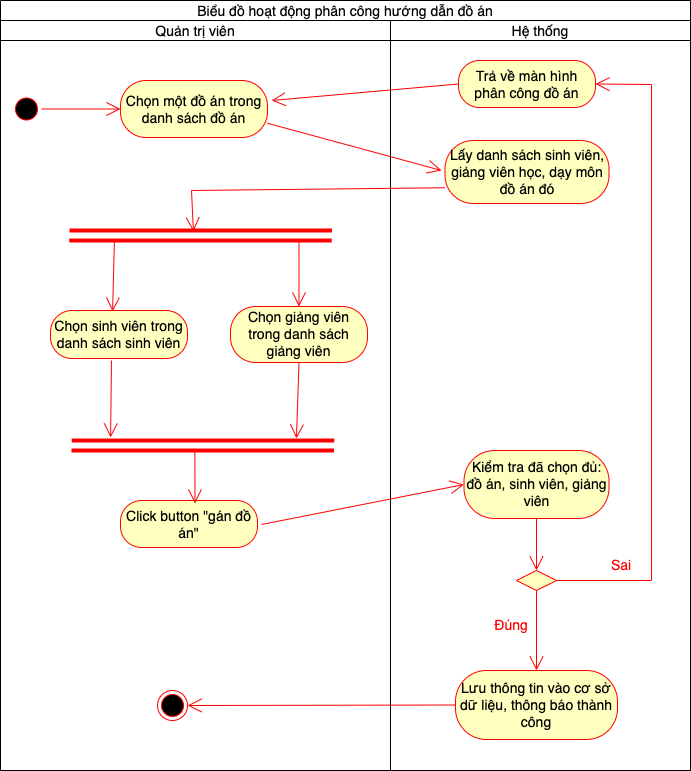
\includegraphics[width=0.75\linewidth]{Figure/qt_assign.png}
    \caption{Sơ đồ hoạt động quy trình nghiệp vụ Phân công hướng dẫn đồ án}
    \label{fig:qt_assign}
\end{figure}

\subsection{Nghiệp vụ Lọc danh sách phân công đồ án}

\begin{figure}[H]
   \centering
    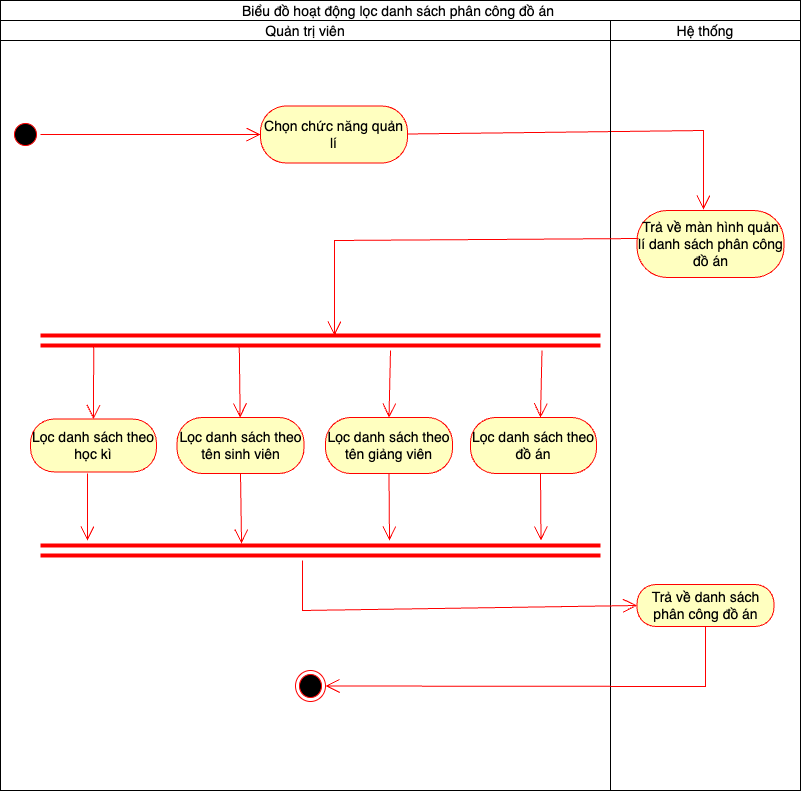
\includegraphics[width=0.75\linewidth]{Figure/loc_ds_do_an.png}
    \caption{Sơ đồ hoạt động quy trình nghiệp vụ Lọc danh sách phân công đồ án}
    \label{fig:loc_ds_do_an}
\end{figure}

\subsection{Nghiệp vụ Xoá phân công hướng dẫn đồ án}
\begin{figure}[H]
   \centering
    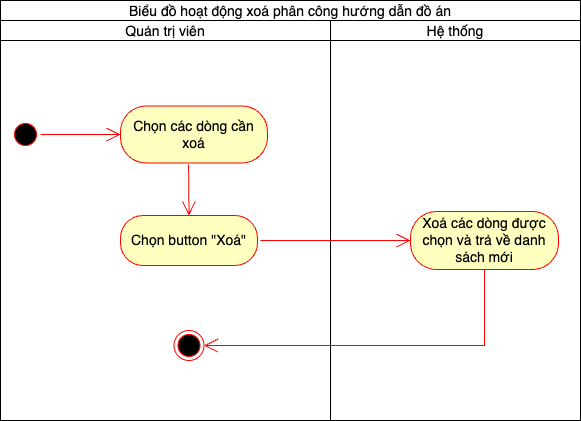
\includegraphics[width=0.75\linewidth]{Figure/delete_assign.png}
    \caption{Sơ đồ hoạt động quy trình nghiệp vụ Xoá phân công hướng dẫn đồ án}
    \label{fig:delete_assign}
\end{figure}
\newpage
\subsection{Nghiệp vụ Xem chi tiết đề tài}

\begin{figure}[H]
   \centering
    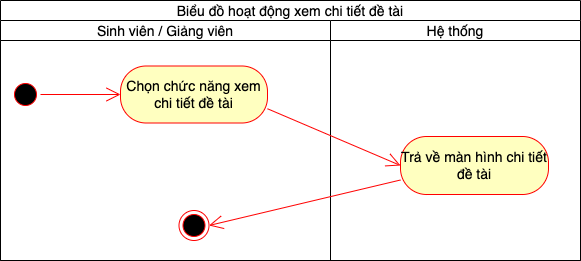
\includegraphics[width=0.75\linewidth]{Figure/detail_topic.png}
    \caption{Sơ đồ hoạt động quy trình nghiệp vụ Xem chi tiết đề tài}
    \label{fig:detail_topic}
\end{figure}

\subsection{Nghiệp vụ Xem danh sách đồ án đang hướng dẫn}
\begin{figure}[H]
   \centering
    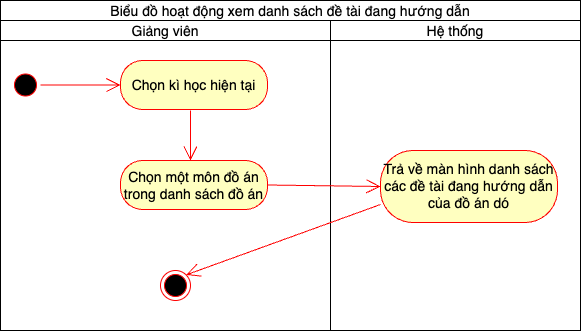
\includegraphics[width=0.75\linewidth]{Figure/ds_de_tai_dang_hd.png}
    \caption{Sơ đồ hoạt động quy trình nghiệp vụ Xem danh sách đồ án đang hướng dẫn}
    \label{fig:ds_de_tai_dang_hd}
\end{figure}

\subsection{Nghiệp vụ Đăng xuất}
\begin{figure}[H]
   \centering
    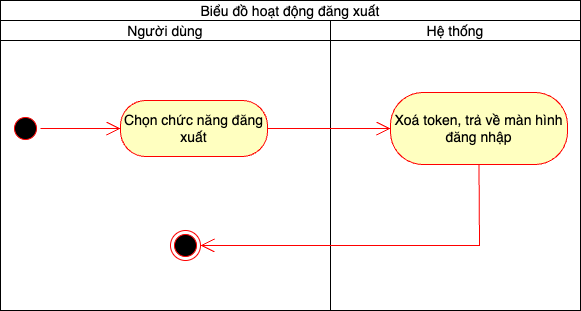
\includegraphics[width=0.75\linewidth]{Figure/dang_xuat.png}
    \caption{Sơ đồ hoạt động quy trình nghiệp vụ Đăng xuất}
    \label{fig:dang_xuat}
\end{figure} 
\section{Đặc tả ca chức năng}

\subsection{Đặc tả use case Đăng nhập}

\begin{table}[H]
\centering
\bgroup
 \raggedleft
\renewcommand{\arraystretch}{1.6}%
% Please add the following required packages to your document preamble:

% \usepackage{multirow}
%\begin{tabular}{| c | L{0.3\linewidth} | L{0.3\linewidth} | L{0.3\linewidth} |}
\begin{tabular}{|L{0.15\linewidth}|L{0.1\linewidth}|L{0.15\linewidth}|L{0.45\linewidth}|}
%{| c | L{0.3\linewidth} | L{0.3\linewidth} | L{0.3\linewidth} |}
\hline

\textbf{Mã use case}                                                                       
& \multicolumn{1}{L{0.1\linewidth}|}{UC01}                                                               
& \multicolumn{1}{L{0.15\linewidth}|}{\textbf{Tên use case}}                                                  
&  Đăng nhập                                                                                                                                       \\ \hline

\textbf{Tác nhân}                                                                         
& \multicolumn{3}{l|}{Sinh viên / giảng viên / quản trị viên}                                                                                                                                                                                                                                                                              \\ \hline

\textbf{Tiền điều  kiện}                         
& \multicolumn{3}{l|}{Đã có tài khoản}                                                                                                                                                                                                                                                                                                     \\ \hline

\textbf{Mục đích sử  dụng}                       
& \multicolumn{3}{p{0.75\linewidth}|}{ Cho phép đăng nhập vào hệ thống và sử dụng các chức năng tương ứng với  từng vai trò}                                                                                                                                                                                      \\ \hline

\textbf{Sự kiện kích hoạt}                      
& \multicolumn{3}{l|}{Không}                                                                                                                                                                                                                                                                                                                    \\ \hline

\multirow{7}{\linewidth}{\textbf{Luồng hoạt động chính}} 
& \multicolumn{1}{L{0.1\linewidth}|}{\textbf{Thứ tự thao tác}} & \multicolumn{1}{L{0.15\linewidth}|}{\textbf{Được thực hiện bởi}} & \textbf{Hành động}                                                                                                                              \\ \cline{2-4} 

& \multicolumn{1}{c|}{1.}                                                                 
& \multicolumn{1}{l|}{Hệ thống}                                                               
& Kiểm tra token đã tồn tại hay chưa                                                                                                              \\ \cline{2-4} 

& \multicolumn{1}{c|}{2.}                                                                  
& \multicolumn{1}{l|}{Người dùng}                                                             
& Điền thông tin đăng nhập                                                                                                                        \\ \cline{2-4} 
& \multicolumn{1}{c|}{3.}                                                                  
& \multicolumn{1}{l|}{Người dùng}                                                             
& Gửi yêu cầu đăng nhập                                                                                                                           \\ \cline{2-4} 

& \multicolumn{1}{c|}{4.}                                                                  
& \multicolumn{1}{l|}{Hệ thống}                                                               
& Kiểm tra dữ liệu đầu vào                                                                                                                        \\ \cline{2-4} 
& \multicolumn{1}{c|}{5.}                                                                  
& \multicolumn{1}{l|}{Hệ thống}                                                               
& Kiểm tra tài khoản có tồn tại hay không, kiểm tra quyền là sinh viên hay giảng viên hay quản trị viên \\ \cline{2-4} 

& \multicolumn{1}{c|}{6.}                                                                  
& \multicolumn{1}{l|}{Hệ thống}                                                               
& Chuyển hướng đến trang chủ ứng có giao diện phù hợp với quyền của người dùng                    \\ \hline

\multirow{3}{\linewidth}{\textbf{Sự kiện thay thế}}      
& \multicolumn{1}{c|}{1a.}                                                                 
& \multicolumn{1}{l|}{Hệ thống}                                                               
& Trả về màn hình trang chủ                                                                                                                   \\ \cline{2-4} 

& \multicolumn{1}{c|}{4a.}                                                                
& \multicolumn{1}{l|}{Hệ thống}                                                               
& Thông báo lỗi: Mời người dùng nhập đầy đủ các trường                                               \\ \cline{2-4} 

& \multicolumn{1}{c|}{5a.}                                                                 
& \multicolumn{1}{l|}{Hệ thống}                                                               
&Thông báo lỗi: Đăng nhập không thành công                                                                                                       \\ \hline

\textbf{Hậu điều kiện}                                                                     
& \multicolumn{3}{l|}{Trả về màn hình trang chủ}                                                                                                                                                                                                                                                                                       \\ \hline

\end{tabular}
\egroup
\caption{Bảng đặc tả use case Đăng nhâp}
\end{table}
\newpage
Danh sách các trường dữ liệu đầu vào form đăng nhập: 

\begin{table}[H]
\centering
\bgroup
\renewcommand{\arraystretch}{1.6}%
\begin{tabular}{|L{0.1\linewidth}|L{0.15\linewidth}|L{0.18\linewidth}|L{0.1\linewidth}|L{0.12\linewidth}|L{0.15\linewidth}|}

\hline
\textbf{Thứ tự} & \textbf{Trường dữ liệu}                                                   & \textbf{Mô tả} & \textbf{Bắt buộc} & \textbf{Yêu cầu hợp lệ} & \textbf{Ví dụ} \\ \hline
1. \hfill             &Id \hfill & Id của người dùng               & Có                &                         & 20173086       \\ \hline
2.                & Password                                                                  & Mật khẩu               & Có                &                         & hadinh         \\ \hline
\end{tabular}
\egroup
\caption{Bảng dữ liệu đầu vào use case Đăng nhập.}
\end{table}


\subsection{Đặc tả use case Tạo công việc}
\begin{table}[H]
\centering
\bgroup
\renewcommand{\arraystretch}{1.6}%

\begin{tabular}{|L{0.15\linewidth}|L{0.1\linewidth}L{0.15\linewidth}L{0.45\linewidth}|}

\hline

\textbf{Mã use case}                                                                       
& \multicolumn{1}{l|}{UC02}                                                               
& \multicolumn{1}{l|}{\textbf{Tên use case}}                                                  
& Tạo công việc                                                                                                                                       \\ \hline

\textbf{Tác nhân}                                                                         
& \multicolumn{3}{p{0.7\linewidth}|}{Sinh viên / giảng viên}                                                                                                                                                                                                                                                                              \\ \hline

\textbf{Tiền điều  kiện}                         
& \multicolumn{3}{p{0.7\linewidth}|}{Đã đăng nhập hệ thống}                                                                                                                                                                                        \\ \hline

\textbf{Mục đích sử dụng }                       
& \multicolumn{3}{l|}{\begin{tabular}[c]{@{}l@{}}Cho phép người dùng tạo công việc\end{tabular}}                                                                                                                                                                                      \\ \hline

\textbf{Sự kiện kích hoạt}                      
& \multicolumn{3}{l|}{\begin{tabular}[c]{@{}l@{}}Nguời dùng click vào floatting button add  \end{tabular} }                                                                                                                                                                                                                                                                                                                    \\ \hline

\multirow{7}{\linewidth}{\textbf{Luồng hoạt động chính}} & \multicolumn{1}{L{0.1\linewidth}|}{\textbf{Thứ tự thao tác}} & \multicolumn{1}{L{0.15\linewidth}|}{\textbf{Được thực hiện bởi}} & \textbf{Hành động}                                                                                                                              \\ \cline{2-4} 

& \multicolumn{1}{c|}{1.}                                                                 
& \multicolumn{1}{l|}{Người dùng}                                                               
& Nguời dùng click vào floatting button add                                                                                                             \\ \cline{2-4} 

& \multicolumn{1}{c|}{2.}                                                                  
& \multicolumn{1}{l|}{Hệ thống}                                                             
& Chuyển đến trang tạo mới công việc                                                                                                                        \\ \cline{2-4} 
& \multicolumn{1}{c|}{3.}                                                                  
& \multicolumn{1}{l|}{Người dùng}                                                             
&  Điền các thông tin trong trang tạo mới                                                                                                                         \\ \cline{2-4} 

& \multicolumn{1}{c|}{4.}                                                                  
& \multicolumn{1}{l|}{Người dùng}                                                             
&  Click vào icon done                                                                                                                         \\ \cline{2-4} 

& \multicolumn{1}{c|}{5.}                                                                  
& \multicolumn{1}{l|}{Hệ thống}                                                               
& Lưu lại thông tin công việc                                                                                                                        \\ \hline    
\textbf{Sự kiện thay thế}                         
& \multicolumn{3}{l|}{Không}                                                                                                                                                                                        \\ \hline                                                                                                   

\textbf{Hậu điều kiện}                                                                     
& \multicolumn{3}{p{0.7\linewidth}|}{Thêm một công việc mới và cập nhật lại danh sách các công việc trong trang các công việc 
}                                                                                                                                                                                                                                                                                       \\ \hline
\end{tabular}
\egroup
\caption{Bảng đặc tả use case Tạo công việc.}
\end{table} \newpage

Danh sánh các trường dữ liệu đầu vào form "Tạo công việc"

\begin{table}[H]
\centering
\bgroup
\renewcommand{\arraystretch}{1.6}%

\begin{tabular} { 
  |L{0.06\textwidth}|
L{0.17\textwidth}|L{0.18\textwidth}|L{0.1\textwidth}|L{0.1\textwidth}|L{0.15\textwidth}| }
\hline
\textbf{Thứ  tự} & \textbf{Trường dữ liệu} & \textbf{Mô tả} & \textbf{Bắt  buộc} & \textbf{Yêu cầu  hợp lệ} & \textbf{Ví dụ} \\ \hline
1 & Title & Tên công việc & Có &  & Chỉnh sửa layout login \\ \hline
2 & Description & Mô tả công việc & Không &  & Chỉnh lại font chữ, ảnh \\ \hline
3 & Start\_date & Thời gian bắt đầu thực hiện công việc& Có &  & 2022-04-01 \\ \hline
4 & Due\_date & Thời gian kết thúc công việc & Có &  & 2022-04-08 \\ \hline
5 & Estimate\_time & Thời gian ước tính hoàn thành & Có &  & 16 \\ \hline
6 & Progress & Tiến độ thực hiện công việc & Có &  & 0.8 \\ \hline
7 & User\_post & Người tạo công việc & Có &  & Đinh Thuý Hà \\ \hline
8 & Status & Trạng thái công việc & Có &  & Huỷ \\ \hline
\end{tabular}

\egroup
\caption{Bảng dữ liệu đầu vào use case Tạo công việc.}
\end{table}
\newpage
\subsection{Đặc tả use case Chỉnh sửa công việc}

\begin{table}[H]
\centering
\bgroup
\renewcommand{\arraystretch}{1.6}%

\begin{tabular}{|L{0.15\linewidth}|L{0.1\linewidth}L{0.15\linewidth}L{0.45\linewidth}|}

\hline

\textbf{Mã use case}                                                                       
& \multicolumn{1}{L{0.1\linewidth}|}{UC03}                                                               
& \multicolumn{1}{L{0.15\linewidth}|}{\textbf{Tên use case}}                                                  
& Chỉnh sửa công việc                                                                                                                                       \\ \hline

\textbf{Tác nhân}                                                                         
& \multicolumn{3}{p{0.75\linewidth}|}{Sinh viên / giảng viên}                                                                                                                                                                                                                                                                              \\ \hline

\textbf{Tiền điều kiện}                         
& \multicolumn{3}{l|}{Đã đăng nhập hệ thống}                                                                                                                                                                                        \\ \hline

\textbf{Mục đích sử dụng}                       
& \multicolumn{3}{p{0.75\linewidth}|}{Cho phép người dùng chỉnh sửa công việc}                                                                                                                                                                                      \\ \hline

\textbf{Sự kiện kích hoạt}                      
& \multicolumn{3}{p{0.45\linewidth}|}{Nguời dùng click vào icon edit }                                                                                                                                                                                                                                                                                                                    \\ \hline

\multirow{7}{\linewidth}{\textbf{Luồng hoạt động chính}} & \multicolumn{1}{L{0.1\linewidth}|}{\textbf{Thứ tự thao tác}} & \multicolumn{1}{L{0.15\linewidth}|}{\textbf{Được thực hiện bởi}} & \textbf{Hành động}                                                                                                                              \\ \cline{2-4} 

& \multicolumn{1}{c|}{1.}                                                                 
& \multicolumn{1}{c|}{Người dùng}                                                               
& Nguời dùng click vào icon edit                                                                                                         \\ \cline{2-4} 

& \multicolumn{1}{c|}{2.}                                                                  
& \multicolumn{1}{L{0.15\linewidth}|}{Hệ thống}                                                             
& Chuyển sang chế độ cho phép chỉnh sửa công việc                                                                                                                  \\ \cline{2-4} 
& \multicolumn{1}{c|}{3.}                                                                  
& \multicolumn{1}{L{0.15\linewidth}|}{Người dùng}                                                             
&Điền các thông tin cần chỉnh sửa.                                                                                                  \\ \cline{2-4} 

& \multicolumn{1}{c|}{4.}                                                                  
& \multicolumn{1}{L{0.15\linewidth}|}{Người dùng}                                                             
&  Click vào icon done                                                                                                                         \\ \cline{2-4} 

& \multicolumn{1}{c|}{5.}                                                                  
& \multicolumn{1}{L{0.15\linewidth}|}{Hệ thống}                                                               
& Cập nhật lại thông tin công việc                                                                                                                        \\ \hline    
\textbf{Sự kiện thay thế}                         
& \multicolumn{3}{l|}{Không}                                                                                                                                                                                        \\ \hline                                                                                                   

\textbf{Hậu điều kiện}                                                                     
& \multicolumn{3}{p{0.75\linewidth}|}{ Người dùng cập nhật lại công việc thành công.
}                                                                                                                                                                                                                                                                                      \\ \hline
\end{tabular}
\egroup
\caption{Bảng đặc tả use case Chỉnh sửa công việc.}
\end{table}
\newpage
Danh sánh các trường dữ liệu đầu vào form "Chỉnh sửa công việc" 

\begin{table}[H]
\centering
\bgroup
\renewcommand{\arraystretch}{1.6}%

\begin{tabular} 
  { 
  |L{0.06\textwidth}|
L{0.2\textwidth}|L{0.18\textwidth}|L{0.1\textwidth}|L{0.1\textwidth}|L{0.2\textwidth}| }
\hline
\textbf{Thứ  tự} & \textbf{Trường dữ liệu} & \textbf{Mô tả} & \textbf{Bắt  buộc} & \textbf{Yêu cầu  hợp lệ} & \textbf{Ví dụ} \\ \hline
1 & Title & Tên công việc & Có &  & Chỉnh sửa layout login \\ \hline
2 & Description & Mô tả công việc & Không &  & Chỉnh lại font chữ, ảnh \\ \hline
3 & Start\_date & Thời gian bắt đầu thực hiện công việc& Có &  & 2022-04-01 \\ \hline
4 & Due\_date & Thời gian kết thúc công việc & Có &  & 2022-04-08 \\ \hline
5 & Estimate\_time & Thời gian ước tính hoàn thành & Có &  & 16 \\ \hline
6 & Progress & Tiến độ thực hiện công việc & Có &  & 0.8 \\ \hline
7 & User\_post & Người tạo công việc & Có &  & Đinh Thuý Hà \\ \hline
8 & Status & Trạng thái công việc & Có &  & Huỷ \\ \hline
\end{tabular}

\egroup
\caption{Bảng dữ liệu đầu vào use case Chỉnh sửa công việc.}
\end{table}
\newpage
\subsection{Đặc tả use case Bình luận công việc}

\begin{table}[H]
\centering
\bgroup
\renewcommand{\arraystretch}{1.6}%

\begin{tabular}{|L{0.15\linewidth}|L{0.1\linewidth}L{0.15\linewidth}L{0.45\linewidth}|}

\hline

\textbf{Mã use case}                                                                       
& \multicolumn{1}{L{0.1\linewidth}|}{UC04}                                                               
& \multicolumn{1}{L{0.15\linewidth}|}{\textbf{Tên use case}}                                                  
& Bình luận công việc                                                                                                                                       \\ \hline

\textbf{Tác nhân}                                                                         
& \multicolumn{3}{p{0.75\linewidth}|}{Sinh viên / giảng viên}                                                                                                                                                                                                                                                                              \\ \hline

\textbf{Tiền điều kiện}                         
& \multicolumn{3}{p{0.75\linewidth}|}{Đã đăng nhập hệ thống}                                                                                                                                                                                        \\ \hline

\textbf{Mục đích sử dụng}                       
& \multicolumn{3}{p{0.75\linewidth}|}{Cho phép người dùng chỉnh sửa công việc}                                                                                                                                                                                      \\ \hline

\textbf{Sự kiện kích hoạt}                      
& \multicolumn{3}{p{0.75\linewidth}|}{Nguời dùng click vào icon edit }                                                                                                                                                                                                                                                                                                                    \\ \hline

\multirow{7}{\linewidth}{\textbf{Luồng hoạt động chính}} & \multicolumn{1}{L{0.1\linewidth}|}{\textbf{Thứ tự thao tác}} & \multicolumn{1}{L{0.15\linewidth}|}{\textbf{Được thực hiện bởi}} & \textbf{Hành động}                                                                                                                              \\ \cline{2-4} 

& \multicolumn{1}{c|}{1.}                                                                 
& \multicolumn{1}{l|}{Người dùng}                                                               
& Nguời dùng click vào icon edit                                                                                                       \\ \cline{2-4} 

& \multicolumn{1}{c|}{2.}                                                                  
& \multicolumn{1}{l|}{Hệ thống}                                                             
&  Chuyển sang chế độ cho phép chỉnh sửa công việc                                                                                                                       \\ \cline{2-4} 
& \multicolumn{1}{c|}{3.}                                                                  
& \multicolumn{1}{l|}{Người dùng}                                                             
&  Điền các thông tin cần chỉnh sửa.                                                                                                                          \\ \cline{2-4} 

& \multicolumn{1}{c|}{4.}                                                                  
& \multicolumn{1}{l|}{Người dùng}                                                             
&  Click vào icon done                                                                                                                          \\ \cline{2-4} 

& \multicolumn{1}{c|}{5.}                                                                  
& \multicolumn{1}{l|}{Hệ thống}                                                               
& Cập nhật lại thông tin công việc                                                                                                                        \\ \hline    
\textbf{Sự kiện thay thế}                         
& \multicolumn{3}{l|}{Không}                                                                                                                                                                                        \\ \hline                                                                                                   

\textbf{Hậu điều kiện}                                                                     
& \multicolumn{3}{p{0.75\linewidth}|}{Người dùng cập nhật lại công việc thàng công. 
}                                                                                                                                                                                                                                                                                      \\ \hline
\end{tabular}
\egroup
\caption{Bảng đặc tả use case Bình luận công việc.}
\end{table}

Danh sách các trường dữ liệu đầu vào 1 bình luận

\begin{table}[H]
\centering
\bgroup
\renewcommand{\arraystretch}{1.5}%
\begin{tabular}{ 
  |L{0.1\textwidth}|
L{0.15\textwidth}|L{0.24\textwidth}|L{0.1\textwidth}|L{0.11\textwidth}|L{0.1\textwidth}| }
\hline
\textbf{Thứ tự} & \textbf{Trường dữ liệu}                                                   & \textbf{Mô tả} & \textbf{Bắt buộc} & \textbf{Yêu cầu hợp lệ} & \textbf{Ví dụ} \\ \hline

1. & content & Nội dung bình luận& Có && hadinh         \\ \hline
2. & file\_name & Tên file đính kèm & Không && hadinh         \\ \hline
3. & file\_path & Đường dẫn file đính kèm & Không && hadinh         \\ \hline

\end{tabular}
\egroup
\caption{Bảng dữ liệu đầu vào use case Bình luận công việc.}
\end{table}

\newpage
\subsection{Đặc tả use case Xem file đính kèm}

\begin{table}[H]
\centering
\bgroup
\renewcommand{\arraystretch}{1.6}%

\begin{tabular}{|L{0.15\linewidth}|L{0.1\linewidth}L{0.15\linewidth}L{0.45\linewidth}|}

\hline

\textbf{Mã use case}                                                                       
& \multicolumn{1}{L{0.1\linewidth}|}{UC05}                                                               
& \multicolumn{1}{L{0.15\linewidth}|}{\textbf{Tên use case}}                                                  
& Xem file đính kèm                                                                                                                                      \\ \hline

\textbf{Tác nhân}                                                                         
& \multicolumn{3}{l|}{Sinh viên / giảng viên}                                                                                                                                                                                                                                                                              \\ \hline

\textbf{Tiền điều kiện}                         
& \multicolumn{3}{p{0.75\linewidth}|}{Đã đăng nhập hệ thống}                                                                                                                                                                                        \\ \hline

\textbf{Mục đích sử dụng}                       
& \multicolumn{3}{p{0.75\linewidth}|}{Cho phép người dùng xem file đính kèm và thao tác với file}                                                                                                                                                                                      \\ \hline

\textbf{Sự kiện kích hoạt}                      
& \multicolumn{3}{p{0.75\linewidth}|}{Nguời dùng click một file trong bình luận   }                                                                                                                                                                                                                                                                                                                    \\ \hline

\multirow{7}{\linewidth}{\textbf{Luồng hoạt động chính}} & \multicolumn{1}{L{0.1\linewidth}|}{\textbf{Thứ tự thao tác}} & \multicolumn{1}{L{0.15\linewidth}|}{\textbf{Được thực hiện bởi}} & \textbf{Hành động}                                                                                                                              \\ \cline{2-4} 

& \multicolumn{1}{c|}{1.}                                                                 
& \multicolumn{1}{L{0.15\linewidth}|}{Người dùng}                                                               
& Nguời dùng click một file trong phần bình luận                                                                                                             \\ \cline{2-4} 

& \multicolumn{1}{c|}{2.}                                                                  
& \multicolumn{1}{L{0.15\linewidth}|}{Hệ thống}                                                             
& Trả về màn hình xem nội dung file                                                                                                                       \\ \cline{2-4} 
& \multicolumn{1}{c|}{3.}                                                                  
& \multicolumn{1}{L{0.15\linewidth}|}{Người dùng}                                                             
&  Có thể thực hiện các thao tác: phóng to, thu nhỏ nội dung, tải file                                                                                                                           \\ \cline{2-4} 

& \multicolumn{1}{c|}{4.}                                                                  
& \multicolumn{1}{L{0.15\linewidth}|}{Hệ thống}                                                             
&  Kiểm tra hành động của người dùng có phải tải file hay không                                                                                                                  \\ \cline{2-4} 

& \multicolumn{1}{c|}{5.}                                                                  
& \multicolumn{1}{L{0.15\linewidth}|}{Hệ thống}                                                               
&Trả về nội dung được phóng to hoặc thu nhỏ                                                                                                                      \\ \hline    
\textbf{Sự kiện thay thế} &
  \multicolumn{1}{c|}{4a.} &
  \multicolumn{1}{L{0.15\linewidth}|}{Hệ thống} &
Thông báo: Tải file thành công khi file đã được tải về máy \\ \hline

\textbf{Hậu điều kiện}                                                                     
& \multicolumn{3}{p{0.75\linewidth}|}{ Người dùng xem file và thao tác với file thành công. 
}                                                                                                                                                                                                                                                                                    \\ \hline
\end{tabular}
\egroup
\caption{Bảng đặc tả use case Xem file đính kèm.}
\end{table} \newpage
\subsection{Đặc tả use case Xoá thông báo đồ án đã đọc}

\begin{table}[H]
\centering
\bgroup
\renewcommand{\arraystretch}{1.6}%

\begin{tabular}{|L{0.15\linewidth}|L{0.1\linewidth}L{0.15\linewidth}L{0.45\linewidth}|}
\hline
\textbf{Mã use case} & \multicolumn{1}{L{0.1\linewidth}|}{UC06} & \multicolumn{1}{L{0.15\linewidth}|}{\textbf{Tên use case}} & Xoá thông báo đồ án đã đọc \\ \hline
\textbf{Tác nhân} & \multicolumn{3}{p{0.75\linewidth}|}{Giảng viên} \\ \hline
\textbf{Tiền điều kiện} & \multicolumn{3}{p{0.75\linewidth}|}{Đã đăng nhập vào hệ thống} \\ \hline
\textbf{Mục đích sử dụng} & \multicolumn{3}{p{0.75\linewidth}|}{Cho phép người dùng xoá danh sách thông báo về đồ án đã đọc} \\ \hline
\textbf{Sự kiện kích hoạt} & \multicolumn{3}{p{0.75\linewidth}|}{Người dùng chọn chức năng xoá thông báo đồ án đã đọc} \\ \hline
\multirow{3}{\linewidth}{\textbf{Luồng hoạt động chính}} & \multicolumn{1}{L{0.1\linewidth}|}{\textbf{Thứ tự thao tác}} & \multicolumn{1}{L{0.15\linewidth}|}{\textbf{Được thực hiện bởi}} & \textbf{Hành động} \\ \cline{2-4} 
 & \multicolumn{1}{c|}{1.} & \multicolumn{1}{L{0.15\linewidth}|}{Người dùng} & Click vào icon xoá \\ \cline{2-4} 
 & \multicolumn{1}{c|}{2.} & \multicolumn{1}{L{0.15\linewidth}|}{Hệ thống} & Lấy danh sách thông báo đồ án người dùng đã đọc . Xoá danh sách đấy trong cơ sở dữ liệu \\ \hline
\textbf{Sự kiện thay thế} & \multicolumn{3}{l|}{Không} \\ \hline
\textbf{Hậu điều kiện} & \multicolumn{3}{p{0.75\linewidth}|}{Xoá thành công danh sách đồ án đã đọc, trả về danh sách các thông báo đồ án chưa đọc} \\ \hline
\end{tabular}

\egroup
\caption{Bảng đặc tả use case Xoá thông báo đồ án đã đọc.}
\end{table}
\newpage
\subsection{Đặc tả use case Tạo lịch gặp sinh viên}

\begin{table}[H]
\centering
\bgroup
\renewcommand{\arraystretch}{1.6}%

\begin{tabular}{|L{0.15\linewidth}|L{0.1\linewidth}L{0.15\linewidth}L{0.45\linewidth}|}
\hline
\textbf{Mã use case} & \multicolumn{1}{L{0.1\linewidth}|}{UC07} & \multicolumn{1}{L{0.15\linewidth}|}{\textbf{Tên use case}} & Tạo lịch gặp sinh viên \\ \hline

\textbf{Tác nhân} & \multicolumn{3}{p{0.75\linewidth}|}{Giảng viên} \\ \hline
\textbf{Tiền điều kiện} & \multicolumn{3}{p{0.75\linewidth}|}{Đã đăng nhập vào hệ thống} \\ \hline
\textbf{Mục đích sử dụng} & \multicolumn{3}{p{0.75\linewidth}|}{Cho phép người dùng tạo lịch gặp mặt sinh viên} \\ \hline

\textbf{Sự kiện kích hoạt} & \multicolumn{3}{p{0.75\linewidth}|}{Người dùng chọn chức tạo lịch gặp sinh viên} \\ \hline
\multirow{6}{\linewidth}{\textbf{Luồng hoạt động chính}} & \multicolumn{1}{L{0.1\linewidth}|}{\textbf{Thứ tự thao tác}} & \multicolumn{1}{L{0.15\linewidth}|}{\textbf{Được thực hiện bởi}} & \textbf{Hành động} \\ \cline{2-4} 

 & \multicolumn{1}{c|}{1.} & \multicolumn{1}{L{0.15\linewidth}|}{Người dùng} &  Click vào icon add trong thẻ lịch hôm nay \\ \cline{2-4} 
 & \multicolumn{1}{c|}{2.} & \multicolumn{1}{L{0.15\linewidth}|}{Hệ thống} & Hiện thị form tạo lịch gặp sinh viên \\ \cline{2-4} 
 & \multicolumn{1}{c|}{3.} & \multicolumn{1}{L{0.15\linewidth}|}{Người dùng} & Điển đầy đủ thông tin vào form, chọn button "OK" \\ \cline{2-4} 
 & \multicolumn{1}{c|}{4.} & \multicolumn{1}{L{0.15\linewidth}|}{Hệ thống} & Lưu thông tin vào cơ sở dữ liệu, \\ \cline{2-4} 
 & \multicolumn{1}{c|}{5.} & \multicolumn{1}{L{0.15\linewidth}|}{Hệ thống} & Quay lại màn hình trang chủ. Thêm lịch gặp sinh viên vào danh sách lịch hôm nay\\ \hline
\textbf{Sự kiện thay thế} & \multicolumn{3}{p{0.75\linewidth}|}{Không} \\ \hline
\textbf{Hậu điều kiện} & \multicolumn{3}{p{0.75\linewidth}|}{Tạo thành công lịch gặp sinh viên và hiển thị trong danh sách lịch hôm nay} \\ \hline
\end{tabular}

\egroup
\caption{Bảng đặc tả use case Tạo lịch gặp sinh viên.}
\end{table}
\newpage
Danh sách đầu vào form "Tạo lịch gặp sinh viên"

\begin{table}[H]
\centering
\bgroup
\renewcommand{\arraystretch}{1.6}%

\begin{tabular} { 
  |L{0.06\textwidth}|
L{0.18\textwidth}|L{0.2\textwidth}|L{0.05\textwidth}|L{0.12\textwidth}|L{0.15\textwidth}| }
\hline
\textbf{Thứ  tự} & \textbf{Trường dữ liệu} & \textbf{Mô tả} & \textbf{Bắt  buộc} & \textbf{Yêu cầu  hợp lệ} & \textbf{Ví dụ} \\ \hline
1 & Title & Tên sự kiện & Có &  & Hẹn gặp trao đổi Project 1 \\ \hline
2 & Name\_student & Tên sinh viên cần gặp & Có & & Giáp Ngọc Hiếu \\ \hline
3 & Date & Thời gian gặp sinh viên& Có &  & 2022-04-01 \\ \hline
4 & Start\_time & Giờ bắt đầu trao đổi với sinh viên & Có &  & 09:00 \\ \hline
5 & End\_time & Giờ kết thúc quá trình trao đổi & Có &  & 09:30 \\ \hline

\end{tabular}

\egroup
\caption{Bảng dữ liệu đầu vào use case Tạo lịch gặp sinh viên.}
\end{table}
\newpage
\subsection{Đặc tả use case Xem danh sách đề tài đang hướng dẫn} 

\begin{table}[H]
\centering
\bgroup
\renewcommand{\arraystretch}{1.5}%

\begin{tabular}{|L{0.15\linewidth}|L{0.1\linewidth}L{0.15\linewidth}L{0.45\linewidth}|}
\hline
\textbf{Mã use case} & \multicolumn{1}{L{0.1\linewidth}|}{UC08} & \multicolumn{1}{L{0.15\linewidth}|}{\textbf{Tên use case}} & Xem danh sách đề tài đang hướng dẫn \\ \hline
\textbf{Tác nhân} & \multicolumn{3}{l|}{Giảng viên} \\ \hline
\textbf{Tiền điều kiện} & \multicolumn{3}{p{0.75\linewidth}|}{Đã đăng nhập vào hệ thống} \\ \hline
\textbf{Mục đích sử dụng} & \multicolumn{3}{p{0.75\linewidth}|}{Cho phép người dùng xem danh sách đề tài đang hướng dẫn và có thể xem chi tiết đề tài} \\ \hline
\textbf{Sự kiện kích hoạt} & \multicolumn{3}{p{0.75\linewidth}|}{Chọn kì học hiện tại} \\ \hline
\multirow{5}{\linewidth}{\textbf{Luồng hoạt động chính}} & \multicolumn{1}{L{0.1\linewidth}|}{\textbf{Thứ tự thao tác}} & \multicolumn{1}{L{0.15\linewidth}|}{\textbf{Được thực hiện bởi}} & \textbf{Hành động} \\ \cline{2-4} 
 & \multicolumn{1}{c|}{1.} & \multicolumn{1}{L{0.15\linewidth}|}{Người dùng} & Click chọn kì học hiện tại \\ \cline{2-4} 
 & \multicolumn{1}{c|}{2.} & \multicolumn{1}{L{0.15\linewidth}|}{Hệ thống} & Trả về danh sách đồ án đang hướng dẫn trong kì học đã chọn\\ \cline{2-4} 
 & \multicolumn{1}{c|}{3.} & \multicolumn{1}{L{0.15\linewidth}|}{Người dùng} & Chọn một môn đồ án bất kì trong danh sách\\ \cline{2-4} 
 & \multicolumn{1}{c|}{4.} & \multicolumn{1}{L{0.15\linewidth}|}{Hệ thống} & Chuyển hướng đến màn hình danh sách các đề tài đang hướng dẫn của đồ án đó \\ \hline
\textbf{Sự kiện thay thế} & \multicolumn{3}{p{0.75\linewidth}|}{Không} \\ \hline
\textbf{Hậu điều kiện} & \multicolumn{3}{p{0.75\linewidth}|}{Hệ thống hiển thị danh sách các đề tài đang hướng dẫn của đồ án} \\ \hline
\end{tabular}

\egroup
\caption{Bảng đặc tả use case Xem danh sách đề tài đang hướng dẫn.}
\end{table}

\newpage
\subsection{Đặc tả use case Xem chi tiết đề tài}

\begin{table}[H]
\centering
\bgroup
\renewcommand{\arraystretch}{1.6}%

\begin{tabular}{|L{0.15\linewidth}|L{0.1\linewidth}L{0.15\linewidth}L{0.45\linewidth}|}
\hline
\textbf{Mã use case} & \multicolumn{1}{L{0.1\linewidth}|}{UC09} & \multicolumn{1}{L{0.15\linewidth}|}{\textbf{Tên use case}} & Xem chi tiết đề tài \\ \hline
\textbf{Tác nhân} & \multicolumn{3}{p{0.75\linewidth}|}{Sinh viên / Giảng viên} \\ \hline
\textbf{Tiền điều kiện} & \multicolumn{3}{p{0.75\linewidth}|}{Đã đăng nhập vào hệ thống} \\ \hline
\textbf{Mục đích sử dụng} & \multicolumn{3}{p{0.75\linewidth}|}{Cho phép người dùng xem thông tin chi tiết về đề tài như : tên đề tài, mô tả để tài, thời gian thực hiện đề tài, thông tin giảng viên hướng dẫn, thông tin sinh viên thực hiện.} \\ \hline
\textbf{Sự kiện kích hoạt} & \multicolumn{3}{p{0.75\linewidth}|}{Người dùng click vào button chi tiết trong thẻ đề tài} \\ \hline
\multirow{3}{\linewidth}{\textbf{Luồng hoạt động chính}} & \multicolumn{1}{L{0.1\linewidth}|}{\textbf{Thứ tự thao tác}} & \multicolumn{1}{L{0.15\linewidth}|}{\textbf{Được thực hiện bởi}} & \textbf{Hành động} \\ \cline{2-4} 
 & \multicolumn{1}{c|}{1.} & \multicolumn{1}{L{0.15\linewidth}|}{Người dùng} & Click vào button chi tiết trong thẻ đề tài \\ \cline{2-4} 
 & \multicolumn{1}{c|}{2.} & \multicolumn{1}{L{0.15\linewidth}|}{Hệ thống} & Trả về màn hình chi tiết đề tài với các thông tin của đề tài \\ \hline
\textbf{Sự kiện thay thế} & \multicolumn{3}{p{0.75\linewidth}|}{Không} \\ \hline
\textbf{Hậu điều kiện} & \multicolumn{3}{p{0.75\linewidth}|}{Hệ thống hiển thị danh sách các đề tài đang hướng dẫn của đồ án} \\ \hline
\end{tabular}

\egroup
\caption{Bảng đặc tả use case Xem chi tiết đề tài.}
\end{table}
\newpage
\subsection{Đặc tả use case Phân công hướng dẫn đồ án}

\begin{table}[H]
\centering
\bgroup
\renewcommand{\arraystretch}{1.6}%

\begin{tabular}{|L{0.15\linewidth}|L{0.1\linewidth}L{0.15\linewidth}L{0.45\linewidth}|}
\hline
\textbf{Mã use case} & \multicolumn{1}{L{0.1\linewidth}|}{UC10} & \multicolumn{1}{L{0.15\linewidth}|}{\textbf{Tên use case}} & Phân công hướng dẫn đồ án \\ \hline
\textbf{Tác nhân} & \multicolumn{3}{p{0.75\linewidth}|}{Quản trị viên} \\ \hline
\textbf{Tiền điều kiện} & \multicolumn{3}{p{0.75\linewidth}|}{Đã đăng nhập vào hệ thống} \\ \hline
\textbf{Mục đích sử dụng} & \multicolumn{3}{p{0.75\linewidth}|}{Cho phép người dùng phân công hướng dẫn đồ án} \\ \hline
\textbf{Sự kiện kích hoạt} & \multicolumn{3}{p{0.75\linewidth}|}{Không} \\ \hline
\multirow{7}{\linewidth}{\textbf{Luồng hoạt động chính}} & \multicolumn{1}{L{0.1\linewidth}|}{\textbf{Thứ tự thao tác}} & \multicolumn{1}{L{0.15\linewidth}|}{\textbf{Được thực hiện bởi}} & \textbf{Hành động} \\ \cline{2-4} 
 & \multicolumn{1}{c|}{1.} & \multicolumn{1}{L{0.15\linewidth}|}{Người dùng} & Chọn một môn đồ án trong danh sách đồ án \\ \cline{2-4} 
 & \multicolumn{1}{c|}{2.} & \multicolumn{1}{L{0.15\linewidth}|}{Hệ thống} & Lấy danh dách sinh viên học môn đồ án, giảng viên dạy môn đồ án \\ \cline{2-4} 
 & \multicolumn{1}{c|}{3.} & \multicolumn{1}{L{0.15\linewidth}|}{Người dùng} & Chọn ra sinh viên trong danh sách sinh viên, giảng viên trong danh sách giảng viên \\ \cline{2-4} 
 & \multicolumn{1}{c|}{4.} & \multicolumn{1}{L{0.15\linewidth}|}{Người dùng} & Chọn button "Gán dự án" \\ \cline{2-4} 
 & \multicolumn{1}{c|}{5.} & \multicolumn{1}{L{0.15\linewidth}|}{Hệ thống} & Kiểm tra đã chọn đủ: đồ án, sinh viên, giảng viên \\ \cline{2-4} 
 & \multicolumn{1}{c|}{6} & \multicolumn{1}{L{0.15\linewidth}|}{Hệ thống} & Lưu thông tin vào cơ sở dữ liệu, thông báo thành công\\ \hline
\textbf{Sự kiện thay thế} & \multicolumn{1}{L{0.1\linewidth}|}{5a} & \multicolumn{1}{L{0.15\linewidth}|}{Hệ thống} & Thông báo: Mời bạn chọn đầy đủ 3 trường: đồ án, sinh viên, giảng viên \\ \hline
\textbf{Hậu điều  kiện} & \multicolumn{3}{p{0.75\linewidth}|}{Hệ thống hiển thị danh sách các đề tài đang hướng dẫn  của đồ án} \\ \hline
\end{tabular}

\egroup
\caption{Bảng đặc tả use case Phân công hướng dẫn đồ án.}
\end{table}

\newpage
\subsection{Đặc tả use case Lọc danh sách phân công đồ án}

\begin{table}[H]
\centering
\bgroup
\renewcommand{\arraystretch}{1.6}%

\begin{tabular}{|L{0.15\linewidth}|L{0.1\linewidth}L{0.15\linewidth}L{0.45\linewidth}|}
\hline
\textbf{Mã use case} & \multicolumn{1}{L{0.1\linewidth}|}{UC11} & \multicolumn{1}{L{0.15\linewidth}|}{\textbf{Tên use case}} & Lọc danh sách phân công đồ án \\ \hline
\textbf{Tác nhân} & \multicolumn{3}{p{0.75\linewidth}|}{Quản trị viên} \\ \hline
\textbf{Tiền điều kiện} & \multicolumn{3}{p{0.75\linewidth}|}{Đã đăng nhập vào hệ thống} \\ \hline
\textbf{Mục đích sử dụng} & \multicolumn{3}{p{0.75\linewidth}|}{Cho phép người dùng lọc danh sách phân công đồ án theo tên đồ án, học kì, tên sinh viên, tên giảng viên} \\ \hline
\textbf{Sự kiện kích hoạt} & \multicolumn{3}{p{0.75\linewidth}|}{Chọn chức năng quản lí} \\ \hline
\multirow{5}{\linewidth}{Luồng hoạt động chính} & \multicolumn{1}{L{0.1\linewidth}|}{\textbf{Thứ tự thao tác}} & \multicolumn{1}{L{0.15\linewidth}|}{\textbf{Được thực hiện bởi}} & \textbf{Hành động} \\ \cline{2-4} 
 & \multicolumn{1}{c|}{1.} & \multicolumn{1}{L{0.15\linewidth}|}{Người dùng} & Chọn chức năng quản lí \\ \cline{2-4} 
 & \multicolumn{1}{c|}{2.} & \multicolumn{1}{L{0.15\linewidth}|}{Hệ thống} & Trả về màn hình quản lí \\ \cline{2-4} 
 & \multicolumn{1}{c|}{3.} & \multicolumn{1}{L{0.15\linewidth}|}{Người dùng} & Có thể thực hiện các hành động: chọn kì học, chọn hoặc điền tên sinh viên, chọn hoặc điền tên giảng viên, chọn hoặc điền tên đồ án \\ \cline{2-4} 
 & \multicolumn{1}{c|}{4.} & \multicolumn{1}{L{0.15\linewidth}|}{Hệ thống} & Trả về danh sách phân công đồ án mới \\ \hline
\textbf{Sự kiện thay thế} & \multicolumn{3}{p{0.75\linewidth}|}{Không} \\ \hline
\textbf{Hậu điều kiện} & \multicolumn{3}{p{0.75\linewidth}|}{Hệ thống hiển thị danh sách phân công đồ án tuỳ theo hành động của  người dùng} \\ \hline
\end{tabular}
\egroup
\caption{Bảng đặc tả use case Lọc danh sách phân công đồ án.}
\end{table}
\newpage
\subsection{Đặc tả use case Xoá phân công hướng dẫn đồ án"}

\begin{table}[H]
\centering
\bgroup
\renewcommand{\arraystretch}{1.6}%

\begin{tabular}{|L{0.15\linewidth}|L{0.1\linewidth}L{0.15\linewidth}L{0.45\linewidth}|}
\hline
\textbf{Mã use case} & \multicolumn{1}{L{0.1\linewidth}|}{UC12} & \multicolumn{1}{L{0.15\linewidth}|}{\textbf{Tên use case}} & Xoá phân công hướng dẫn đồ án \\ \hline
\textbf{Tác nhân} & \multicolumn{3}{l|}{Quản trị viên} \\ \hline
\textbf{Tiền điều kiện} & \multicolumn{3}{p{0.75\linewidth}|}{Đã đăng nhập vào hệ thống} \\ \hline
\textbf{Mục đích sử dụng} & \multicolumn{3}{p{0.75\linewidth}|}{Cho phép người dùng xoá phân công đồ án} \\ \hline
\textbf{Sự kiện kích hoạt} & \multicolumn{3}{p{0.75\linewidth}|}{Người dùng tích vào các ô checkbox ở từng hàng} \\ \hline
\multirow{4}{\linewidth}{\textbf{Luồng hoạt động chính}} & \multicolumn{1}{L{0.1\linewidth}|}{\textbf{Thứ tự thao tác}} & \multicolumn{1}{L{0.15\linewidth}|}{\textbf{Được thực hiện bởi}} & \textbf{Hành động} \\ \cline{2-4} 
 & \multicolumn{1}{c|}{1.} & \multicolumn{1}{L{0.15\linewidth}|}{Người dùng} & Tích vào ô checkbox \\ \cline{2-4} 
 & \multicolumn{1}{c|}{2.} & \multicolumn{1}{L{0.15\linewidth}|}{Người dùng} & Click button "Xoá" \\ \cline{2-4} 
 & \multicolumn{1}{c|}{3.} & \multicolumn{1}{L{0.15\linewidth}|}{Hệ thống} & Xoá các dòng được chọn, hiển thị danh sách mới sau khi xoá thành công. \\ \hline
\textbf{Sự kiện thay thế} & \multicolumn{3}{l|}{Không} \\ \hline
\textbf{Hậu điều kiện} & \multicolumn{3}{p{0.75\linewidth}|}{Hệ thống cập nhật danh sách phân công đồ sau khi xoá một số phân công đồ án} \\ \hline
\end{tabular}
\egroup
\caption{Bảng đặc tả use case Xoá danh sách phân công đồ án.}
\end{table}
\newpage
\subsection{Đặc tả use case Đăng xuất}

\begin{table}[H]
\centering
\bgroup
\renewcommand{\arraystretch}{1.6}%

\begin{tabular}{|L{0.15\linewidth}|L{0.1\linewidth}L{0.15\linewidth}L{0.45\linewidth}|}
\hline
\textbf{Mã use case} & \multicolumn{1}{L{0.1\linewidth}|}{UC13} & \multicolumn{1}{L{0.15\linewidth}|}{\textbf{Tên use case}} & Đăng xuất \\ \hline
\textbf{Tác nhân} & \multicolumn{3}{p{0.75\linewidth}|}{Sinh viên/ giảng viên/ quản trị viên} \\ \hline
\textbf{Tiền điều kiện} & \multicolumn{3}{p{0.75\linewidth}|}{Đã đăng nhập vào hệ thống} \\ \hline
\textbf{Mục đích sử dụng} & \multicolumn{3}{p{0.75\linewidth}|}{Cho phép người dùng đăng xuất khỏi hệ thống} \\ \hline
\textbf{Sự kiện kích hoạt} & \multicolumn{3}{p{0.75\linewidth}|}{Người dùng click vào button "Đăng xuất"} \\ \hline
\multirow{3}{\linewidth}{\textbf{Luồng hoạt động chính}} & \multicolumn{1}{L{0.1\linewidth}|}{\textbf{Thứ tự thao tác}} & \multicolumn{1}{L{0.15\linewidth}|}{\textbf{Được thực hiện bởi}} & \textbf{Hành động} \\ \cline{2-4} 
 & \multicolumn{1}{c|}{1.} & \multicolumn{1}{L{0.15\linewidth}|}{Người dùng} & Click button "Đăng xuất" \\ \cline{2-4} 
 & \multicolumn{1}{c|}{2.} & \multicolumn{1}{L{0.15\linewidth}|}{Hệ thống} & Xoá token, trả về màn hình đăng nhập \\ \hline
\textbf{Sự kiện thay thế} & \multicolumn{3}{p{0.75\linewidth}|}{Không} \\ \hline
\textbf{Hậu điều kiện} & \multicolumn{3}{p{0.75\linewidth}|}{Đăng xuất người dùng khỏi hệ thống} \\ \hline
\end{tabular}


\egroup
\caption{Bảng đặc tả use case Đăng xuất.}
\end{table}

\section{Các yêu cầu phi chức năng}
\subsection{Yêu cầu về bảo mật}
Mật khẩu của người dùng phải được mã hoá. Các request lên server phải được đính kèm token.

Sử dụng HTTPS để giao tiếp giữa server và client cho phép trao đổi thông tin một cách an toàn trên internet. 
\subsection{Yêu cầu về hiệu năng}
Thời gian phản hồi chấp nhận được.
\subsection{Yêu cầu về giao diện}
Ngôn ngữ sử dụng là Tiếng Việt, giao diện thân thiện với người dùng.  

%%%%%%%%%%%%%%%%%%%%%%%%%%%%%%%%%%%

\end{document}